\chapter{Pi power}

\notesurl{rpi2}

So far you've used your Pi and a lab machine separately, and hopefully you've come to understand that they are both essentially the same kind of machine; they both run variations of the same operating system, and the principles you learn using one for the most part apply to the other. In the case of the Pi, you have complete control of the device as a super user, so can do absolutely what you like to it; in the case of the lab machines you have access to much more powerful hardware, but more restricted access to the filestore and operating system for reasons of security and privacy. 

Today, we'll be getting your Pi and a desktop PC to communicate with one another, to reinforce the similarities between these setups, and to expose you to some of the principles of networking and remote access. 

\section{The LXDE window manager}

Connect your Pi up to the monitor, keyboard, mouse, network and power supply as before, and log in (remembering this time to use whatever password you set on the Pi rather than your University password, and the username `pi'). At the console, type:

\begin{ttoutenv}
$ startx
\end{ttoutenv}

to start up X Windows and the Pi's default window manager, LXDE, which which appear moments later looking like the screenshot in Figure \ref{figure:lxde-desktop}. 

LXDE (the `Lightweight X11 Desktop Environment') is designed to be a lean, fast desktop environment, which makes it ideally suited for the Pi's modest CPU. Although rather less rich in features and `eyecandy' than Gnome, LXDE is a fully functioning environment that has all the features you will need for operating and programming the Pi. 

Down at the bottom of the screen you will see LXDE's `panel'. On the left of the panel (\protect\circled{1} in the figure) are controls that give you access to various applications, tools and system preferences. On the panel's right (marked \protect\circled{2}) are a CPU meter, a clock, a control that will allow you to lock the Pi's screen temporarily so that you can nip out for a coffee, and the logout button that does what you'd expect a logout button to do. On the desktop itself are shortcuts to some useful applications including a Terminal and Midori, which is a simple web browser. 

Spend a few minutes exploring the GUI. You'll almost certainly find that you're double-clicking on things that only need a single click, and vice versa, and may find that things aren't quite where you expect them to be---but rather than dismissing LXDE as being crude, embrace the differences; you may well find that you come to prefer its `no frills' approach to window management over that of richer, heavier-weight environments such as Gnome. LXDE and other slimmed-down graphical environments consume considerably fewer CPU cycles and hence less power than their richer counterparts, and while this isn't an issue when you're running on a mains-powered desktop machine with a beefy graphics card such as the lab machines, this can be a serious issue for devices running off batteries. 

\begin{figure}
\centerline{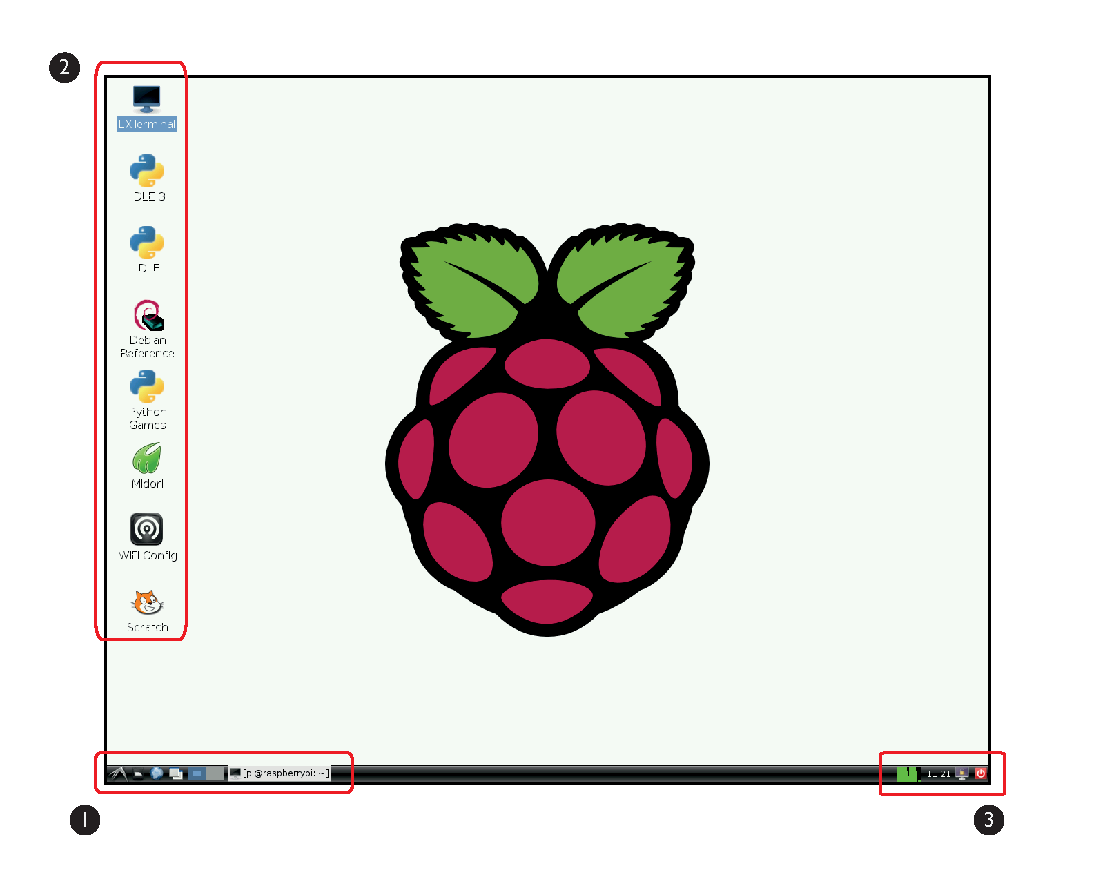
\includegraphics[width=14cm]{images/lxde-desktop}}
\caption{The Pi's default window manager is called LXDE.}\label{figure:lxde-desktop}
\end{figure}

\section{Configure mutt}

Once you've found your way around LXDE, fire up a Terminal so that you can configure your Pi to read your University email using Mutt. Unlike the lab machines, Mutt isn't installed by default on the Pi, so you'll need to do that yourself using:

\begin{ttoutenv}
$ sudo apt-get install mutt
\end{ttoutenv}

Once the install has completed, you'll need to adjust Mutt's settings so that they once again point at your University email account. You could do this by following the instructions in the previous sessions's script again, but there's a much easier way: let's just copy the configuration file you created on the desktop PC last time, over to the Pi. 

First you need to check that you still have the \ttout{.muttrc} configuration file in your home filestore of your Computer Science network account. You \textit{could} unplug all the cables from the Pi, connect them back into the desktop PC and check that way, but that's no fun (especially because we'd then have to reverse it all to do the next bit of the exercise). But you don't need to do that -- you can check remotely. 

So, find the hostname of the lab PC on your desk; there are several ways to do this:

\begin{itemize}
\item If you haven't logged into the PC, then it should be showing a prompt like  \ttout{lf012:}
\item If you're already logged in, but have not started a window manager, your console prompt will be something like  \verb|{[mbasstlh@lf012 ~]$| (where \ttout{mbasstlh} would be replaced by your own username, of course).
\item If you are logged in to the PC and inside a window manager, open a Terminal window. It should show you the command line prompt, as above. You could also type \verb|echo $HOSTNAME|.
\end{itemize}

In the terminal window on the Pi, issue this command:

\begin{ttoutenv}
$ ssh USERNAME@HOSTNAME.cs.man.ac.uk
\end{ttoutenv}

obviously replacing USERNAME with your University username, and HOSTNAME with the name of the PC in front of you. You'll need to enter your university password, and will most likely be presented with text something similar to this:

\begin{ttoutenv}
The authenticity of host 'lf012 (130.88.197.112)' can't be established.
RSA key fingerprint is 20:6d:2d:90:5e:8f:9f:19:39:70:ce:48:a6:93:ec:4c.
Are you sure you want to continue connecting (yes/no)? 
\end{ttoutenv}

Type \ttout{yes} (and hit return) in response to the question. You should then be given a command prompt (you'll learn more about what this message actually means in COMP\ref{securityguffs}, but for now just treat it as something that happens the first time you try to connect to a particular machine). Notice that this command prompt no longer says \ttout{pi@raspberrypi}, but rather has the name of the machine you've just remotely logged into. The \ttout{ssh} command stands for `Secure Shell', and allows you to issue instructions to a remote machine as though you had logged in at that machine's console. 

Type \ttout{ls -a} to confirm that your \fname{.muttrc} file is still where you expect it to be, and if all is well then press Ctrl+D to log out of the remote shell you just started, and you will return to the shell running locally on your Pi (you'll see the command prompt change back to being `pi' again). Now we know the file we want is there, we need to copy it from your Computer Science filestore onto your Pi's local filestore.

To do this, we're going to use the \ttout{scp} (Secure Copy) command, which in some ways behaves like \ttout{cp}, but allows us to move files \textit{between machines}. 

Like \ttout{cp}, the \ttout{scp} command in its basic form takes two parameters, the first is the name of the source file (the one you want to copy), and the second is the name of the destination file (the one you want to create). The difference with \ttout{scp} is that either of these files can be on a remote machine, which means that you need to provide the command with enough information about the location of the remote file in terms of the network and file system, and any login details necessary to get at it. The syntax for providing this information is:

\begin{ttoutenv}
username@hostname:filepath
\end{ttoutenv}

So for example, if you wanted to retrieve a file called \ttout{cheese.jpg} from the home directory of a user called \ttout{mrnoodle} that was stored machine with the host name \ttout{mypc.example.com}, and you wanted the local copy of the file to be called \ttout{mycheese.jpg} the command would be:

\begin{ttoutenv}
$ scp mrnoodle@mypc.example.com:cheese.jpg mycheese.jpg
\end{ttoutenv}

Then, supposing you had edited the file \ttout{mycheese.jpg} on your local machine and wanted to put the file back into the home directory of the mrnoodle account on the remote machine, but under a different name (so as not to over-write the original), you would issue:

\begin{ttoutenv}
$ scp mycheese.jpg mrnoodle@mypc.example.com:newcheese.jpg
\end{ttoutenv}

We're not exactly sure why MrNoodle and cheese feature quite so prominently in these exercises either, just go with the flow. Now use your new-found knowledge of \ttout{scp} to copy the \fname{.muttrc} file from your Computer Science account onto your Pi. Conveniently, there's nothing in the \fname{.muttrc} file that is specific to the Computer Science account setup, so you can use it as-is for Mutt on the Pi. 

Check that the file has copied over successfully using \ttout{less}, and then start up Mutt from a terminal. If everything has gone to plan, you should now be able to read and compose emails on your Pi. You can of course install other mail clients if you want to; there is a version of Thunderbird for the Pi called `icedove' (yes, yet another play on words), or a much leaner graphical client called Claws Mail (which if you want to can be installed using \ttout{sudo apt-get install claws-mail}). Remember, though, that the memory-card we've given you for your Pi is fairly small, so you probably don't want to clutter it up with unnecessary packages, and should find that Mutt is perfectly ok for sending and reading the occasional email. 

\section{X Windows again}

As we mentioned before, the X Windows system is a powerful beast, and although it was designed a long time ago (around 1984), it was in many ways way ahead of its time -- rather like the design of UNIX itself.

Remember that the GUI you're now using on the Pi consists of two systems working together: X Windows (which amongst other things gives software access to the display hardware), and the Window Manager (in this case, LXDE) that provides the WIMP-style features such as movable windows and clickable controls. The X Windows system operates as a Client/Server architecture, where the `server' part does the drawing of stuff onto the screen, and clients request that things be drawn. One of the really nice features of X Windows is that it doesn't care too much about where the requests to draw things come from. Typically they come from processes that are running on the same hardware as the X Server, but this need not be the case as you're about to demonstrate.

Log back in to the lab PC using the \ttout{ssh} command, but this time include a \texttt{-X} switch before your username, like:

\begin{ttoutenv}
$ ssh -X USERNAME@HOSTNAME.cs.man.ac.uk
\end{ttoutenv}

The \ttout{-X} switch (note that it's an uppercase X) tells the \ttout{ssh} program to redirect any X Windows requests back through the network from the remote machine to the X Server running on the local machine.

Confirm that you are indeed logged into your Computer Science account by checking the command prompt and using \ttout{ls} to make sure the files in your home directory are the ones you'd expect, and then type:

\begin{ttoutenv}
$ xeyes
\end{ttoutenv}

Googly eyes that follow the mouse! What's not to like? Well, okay, perhaps not hugely exciting in itself, but what's actually happening here is rather sophisticated. The \ttout{xeyes} program is running on the remote machine machine (the desktop PC); but the instructions to draw its graphical output are being forwarded over the secure shell connection you've made from the Pi to the remote machine, so that the Pi's X Windows system receives them. Press CTRL+C to abort \ttout{xeyes}, and instead try running \ttout{xterm}. You should see a new terminal window appear on your Pi's screen (which probably looks slightly different to the terminal you launch on the Pi a moment ago). This XTerminal, rather like xeyes, is actually running on the desktop machine---only its graphical representation is appearing on your Pi (if you use \texttt{ls} in that terminal, you'll see that its your Computer Science account that's visible, rather than your Pi's filestore). 

How could you use this feature to your advantage to give you a temporary graphical mail client (or perhaps to use Firefox as a web browser, rather than Midori) on the Pi, without needing to install any packages on the Pi itself?

\section{A Simple Web Server}

This next exercise involves setting up a simple web server on the Pi, but before we can do that you'll need to create some basic web pages to display. 

Start up a terminal, and create a directory called \ref{something} your home directory, and in that directory, use Nano to create a file called \fname{index.html} with the following content:

\begin{ttoutenv}
<html>
<body>
Hello world!
</body>
</html>
\end{ttoutenv}

From within that directory, run the command:

\begin{ttoutenv}
python -m SimpleHTTPServer
\end{ttoutenv}

and then use Midori to browse to the following URL:

\begin{ttoutenv}
http://localhost:8000
\end{ttoutenv}

If your browser displays a page saying `Hello World', pat yourself on the back---you've just created a web page \textit{and} set up a simple web server to host it. The URL you used to view this page may look a bit odd compared with others you have seen. The \texttt{http://} part you'll no-doubt be familiar with from other web-addresses that you've seen; the `localhost' part is a convention that means `this machine' (you could for example, \ttout{ping} or \ttout{ssh} a machine called \texttt{localhost}, though neither is a very useful thing to do). The section of the URL that follows \texttt{localhost} may be even less familiar: this is the \textit{port} on which the simple web-server that you've set up is serving web pages; by default web browsers expect servers to operate on port 80, but the \ttout{python -m SimpleHTTPServer} command you used here defaults to port 8000, so we had to add that to the URL. We'll leave the issue of ports there for now, and revisit that in more detail in the 2nd semester in COMP18112. 

\subsection{A slightly more interesting web page}

Now spend a few minutes creating a slightly more interesting web page. You can either use the Nano editor to do this, or find the Pi's default graphical text editor. Create a single page about yourself that contains a paragraph describing who you are, which programme you're on (e.g. Computer Science, Software Engineering, etc.), and which contains a picture of yourself as well as the image you created earlier using Inkscape. 

Don't worry about finely crafted words here---this is really just a way of creating a file that we can get you to edit in various ways a little later on. A few sentences will do, and you can always chance it later. 

As for the photograph of you, we'd ideally like you to use something recent that someone could recognise you by because this will be useful later on for staff and other students. It can be any kind of photo you like; silly or serious, whatever you're comfortable with, but please make sure it doesn't contain anything offensive since it will eventually be visible on the internet. If you're not comfortable with having a photo of yourself on the net, you can use a photo of something else (but you must make sure you have permission to re-use a picture that's not yours; anything you find on Wikipedia should be okay for this purpose, and there will be more guidance on how to use others' photos later in this course). If you didn't have a photo handy, take one with your phone, or ask one of your fellow students to do it for you on theirs.

You've already learned several ways of getting files onto your Pi, but here's a reminder:
\begin{itemize}
\item You could mail the photo to yourself, and use Mutt to save the attachment onto the Pi (more help on how to do this in Breakout \ref{breakout:attachments})
\item If the picture is on the web somewhere, you could use Midori to find and save it. 
\item Alternatively for images on the web, you could use \ttout{curl} to fetch it directly from a URL to a file. 
\item You could use \ttout{scp} to copy it from some other machine directly to your Pi. 
\item Or if all else fails, you could use a USB device to copy it from one place to another (though this isn't entirely trivial on the Pi; see the instructions in Appending \ref{blah}). 
\end{itemize}

If you need guidance on how to write the web page itself, then Appendix \ref{appendix:simplehtml} contains a few pointers; though there are plenty of tutorials on the web as well. 

To finish this exercise, use Midori to check that your web page is displaying correctly.

\section{Headless Pi}

The Pi can be used as a respectable desktop machine, but it really comes into its own as a `server' or controller for other pieces of hardware. In these next few exercises we'll use the Pi in what is called `headless' mode, that is without its own screen and keyboard, to create a proper web server to host your pages. 

At a terminal, type the command \ttout{ifconfig}, short for `interface configuration', which will give you details about the network configuration on the Pi. This will return something along the lines of

\begin{ttoutenv}
eth0      Link encap:Ethernet  HWaddr b8:27:eb:a5:d5:82
          inet addr:192.168.2.2  Bcast:192.168.2.255  Mask:255.255.255.0
          UP BROADCAST RUNNING MULTICAST  MTU:1500  Metric:1
          RX packets:39778 errors:0 dropped:0 overruns:0 frame:0
          TX packets:4338 errors:0 dropped:0 overruns:0 carrier:0
          collisions:0 txqueuelen:1000
          RX bytes:18251497 (17.4 MiB)  TX bytes:651537 (636.2 KiB)

lo        Link encap:Local Loopback
          inet addr:127.0.0.1  Mask:255.0.0.0
          UP LOOPBACK RUNNING  MTU:16436  Metric:1
          RX packets:105 errors:0 dropped:0 overruns:0 frame:0
          TX packets:105 errors:0 dropped:0 overruns:0 carrier:0
          collisions:0 txqueuelen:0
          RX bytes:8550 (8.3 KiB)  TX bytes:8550 (8.3 KiB)
\end{ttoutenv}

This tells you that the Pi has two network devices currently active: one called `eth0', which is the phyiscal ethernet cable you plugged into the device and allows the Pi to communicate with other computers on the network (and in this case, on the internet); and a second one called `lo' which is a `virtual connection' or `local loopback' connection that allows the Pi to route network traffic back to itself (this is how the `localhost' trick you used earlier to look at web pages on the Pi worked). You'll learn a lot more about network configuration in the second year Computer Networks course (COMP28411). 

The thing we're interested in right now is the IP Address that's been allocated to your Pi. Look for the line in the `eth0' block that says `inet addr:' and note down the number that follows this in your logbook (in the case of our example that is 192.168.2.2 but in your case it will probably be something else). Don't worry too much about what this number means or where it came from for now---we'll return to this in COMP18112 in the second semester. For now, just treat this as being a unique number that identifies your Pi on the Computer Science network. 

Quit the graphical environment, and log out of your Pi. Leave the network connection and power supply plugged in, but disconnect the mouse and keyboard, and reconnect them to the desktop PC. Switch the monitor over to display the desktop PC's screen, and log in to that with your University credentials. 

Start up a terminal, and use \ttout{ssh} to log into your Pi:

\begin{ttoutenv}
$ ssh pi@IPADDRESSOFPI
\end{ttoutenv}

replacing IPADDRESSOFPI with the IP Address you noted down a moment ago. Since this is the first time you're logging in from your CS account to your Pi, expect to see the `The authenticity of host' warning again; just say yes to the prompt, and enter your Pi user's password. 

Change directory to the `aboutme' directory you created for your web-page earlier, and re-start the simple Python web server. 

Next, start up Firefox using the keyboard shortcut you created in the previous lab session, and enter the URL:

\begin{ttoutenv}
http://IPADDRESSOFPI:8000
\end{ttoutenv}

and you should see your web page appear, served off your Pi to the desktop machine just like a real web server. Get the person next to you to see if they can see your web page from their machine by using your Pi's address; and return the favour by checking that theirs is also working (it's worth noting that the IP addresses of the Pis are only visible within the School of Computer Science, so pages served off your Pi will not be visible on the wider Internet).

\begin{diversion}
Some information about what's happened when you run python -m SimpleTHingy
\end{diversion}

\subsection{Apache; a proper web server}

The simple Python-based web server that you've been running so far is doing the bare minimum necessary to allow HTML pages to be fetched by a browser. Although it was a handy way of getting you going with web server technology, it's a long way off being the kind of fully-featured web server you would need to run a modern website. Fortunately, the Apache HTTP Server---the software that \textit{is} used to run over half the world's websites---is Open Source and runs quite happily on a Raspberry Pi. You wouldn't want to be powering the next eBay or Facebook from a Pi, but to illustrate the principles, it'll do the job nicely. 

Before we install apache on your Pi, there's a bit of housekeeping to do that will conveniently expose you to a few more Unix concepts that we've rather skated over so far. 

\subsection{Permissions, users and groups}

Right at the beginning of these sessions you logged in to the Pi as a particular user called `pi', and on the desktop machines you've been logging in using your University credentials. It's fairly obvious what the general principles are here---logging in with a username and password is a way of protecting `your stuff' from being seen or messed around with by other users. Roughly speaking this means two things: first, and most obviously, files created by you should be in some sense `owned' by you so that you can control who can see/modify them; second, and perhaps less obviously, processes that you start---whether from the command line or the graphical environment---are also `yours' and have certain privileges/restrictions that are associated with your user. 

For this to work, it means that both the Unix file system and its process management system need to be aware of the notion of a user. Use \ttout{cd} to change to your home directory and issue \ttout{ls -l} to list the files there in what's called `long format' (the \ttout{-l} switch means `give me extra information about each file'). You'll see something like Figure \ref{figure:longformls}.

\begin{figure}
\centerline{\includegraphics[width=14cm]{images/longformls}}
\caption{An example of the `long format' output from ls.}\label{figure:longformls}
\end{figure}

Working from right to left in Figure \ref{figure:longformls}, column \protect\circled{7} contains the filename, column \protect\circled{6} gives the date that the file was last modified (the exact format of the date will vary so as to always be `useful'; older files will have a year instead of an exact time, for example) and column \protect\circled{5} shows the size of the file in bytes. Columns \protect\circled{4} and \protect\circled{3} give the group and user to which the file belongs (often these will appear to be the same name); we'll come back to this in a moment. Column \protect\circled{2} shows the number of links associated with the file (ignore this for now, you'll cover it in \ref{blah}), and finally column \protect\circled{1} gives a synopsis of the file's permissions, which we'll look at again shortly. 

In our example, the file's user (Column \ref{3}) is not surprisingly `pi', which is the username under which you logged in. Run \ttout{ls -l /} (i.e. `long format list of the root directory), and you'll see that the files at the top of the filesystem are owned by a user called \ttout{root}. 

\begin{note}
Some words here about the CS setup, i.e. how users and groups are arranged
\end{note}

